\ifx \allfiles \undefined
\documentclass{article}
\usepackage{booktabs}
\usepackage{multirow}
\usepackage{graphicx}
\usepackage{subfigure}

\begin{document}
\title{Experiments}
\maketitle \else \fi

\newcommand{\at}{\emph{@}}

\section{Experiments}\label{sec:experiment}
In this section, the ranking performance of our proposed four methods, including snowball algorithm (SA), bidirectional snowball algorithm (BSA), naive Bayes algorithm (NBA) and co-training algorithm (CA), is tested on real dataset extracted from twitter. The precision of top $k$ results (precision\at$k$) and recall of top $k$ results (recall\at$k$) are used to evaluate the ranking result. Precision\at$k$ (Recall\at$k$) is the ratio between the number of users that belong to $\mathcal{C}$ in top $k$ results and $k$ (total number of users in $\mathcal{C}$ in the dataset). As the value of recall\at$k$ is proportional to the value of precision\at$k$, the experiment only shows the value of precision@$k$.
%In the experiments, we use precision at the position $K$ to evaluate the accuracy of our ranking result. The precision at the position $K$ measures how many related user we ranked in top $K$ positions. The precision at $K$ method penalizes the model which performs poorly in ranking result. Here we didn't use recall as one of our metrics since that we can hardly obtain the exactly number of users belong to our target category.

\subsection{Experiment Setup}
\textbf{Data collection:} Twenty seed users were selected from each of the four universities, including UCLA, USC, Stanford and MIT. User profile (id, location, screen name, number of followings and followers, and a short biography) of these seed users was crawled using the Twitter API. Starting from these seed users, a two-level breadth first traversal was performed to retrieve their followers and their followers' followers. If a new user from these four universities was discovered during the procedure (the user's biography contains the university name), this user was marked as a seed user and another two-level breadth first traversal starting from this user was performed. The data was collected during October, 2011. The crawler had collected more than 540,000 users and 780,000,000 following relations. It had also collected the most recent 20 tweets for each user, summing up to $15,321,508$ tweets in total. These tweets contain $3,143,115$ different words. After eliminating the words which appear less than $100$ times, there are about $20,000$ words left.

\textbf{Data preprocessing:} Experiment tested different algorithms' ability on discovering users from UCLA, USC, Stanford and MIT. Users in each university were considered as a category. For example, the users in UCLA belongs to category UCLA, and the keyword $z_{\mathcal{C}}$ is the university name ``UCLA''. For each category $\mathcal{C}$, the users were partitioned into two sets $\mathcal{A}$ and $\mathcal{B}$ based on whether $z_{\mathcal{C}}$ appeared in their biographies. We randomly selected $20\%$ users in $\mathcal{A}$, removed the biography of these users, and moved them to $\mathcal{B}$.
%During our experiments, we mainly focus on ranking users from four categories, they are UCLA, Stanford, MIT and USC. The user belong to these four universities may highly connected with each other. Later in our experiments part, we will prove that some of our algorithm will still have good performance with dataset that is not highly connected. For category of each university, we use $80\%$ users with target keyword in their short bio as training data and erase the target keyword appeared in other $20\%$ users.

\textbf{Data labeling:} Top 100 results of BSA, NBA and CA from UCLA category are manually labeled. The labeling process considers the user's biography, location, tweets, following relations, and the search result from Google using the user's name as keyword. This process tries to discover as many UCLA users as possible.
%In the evaluation process, we will also label top $100$ results of different approaches from UCLA category by human in order to obtain a more accuracy evaluation result. During the labeling process, we take into consideration not only users' profile information, but also users' tweets, users' following relationship and search users' names in Google. Besides, as we present a ranking result, we will consider whether a user never log on twitter after he register his account and we may separate user who is belong to this category and who is interest in this category. More detail information about labeling result will discuss in the discussion section.

\subsection{Ranking Performance}
This part of experiment evaluated the precision\at$k$ for different algorithms. The algorithm worked on the processed user sets $\mathcal{A}$ and $\mathcal{B}$, while the evaluation is done on the original dataset. A user which has keyword $z_{\mathcal{C}}$ in his biography belongs to $\mathcal{C}$, otherwise he does not belong to $\mathcal{C}$.
%In this part of the experiments, we use our label data and sort the users with respect to the estimated relevance given by our algorithm. 
The precision\at$k$ curves of different methods on different categories are shown in Figure~\ref{fig:e1}.

\begin{figure*}[htbp]
\centering
\subfigure[UCLA]{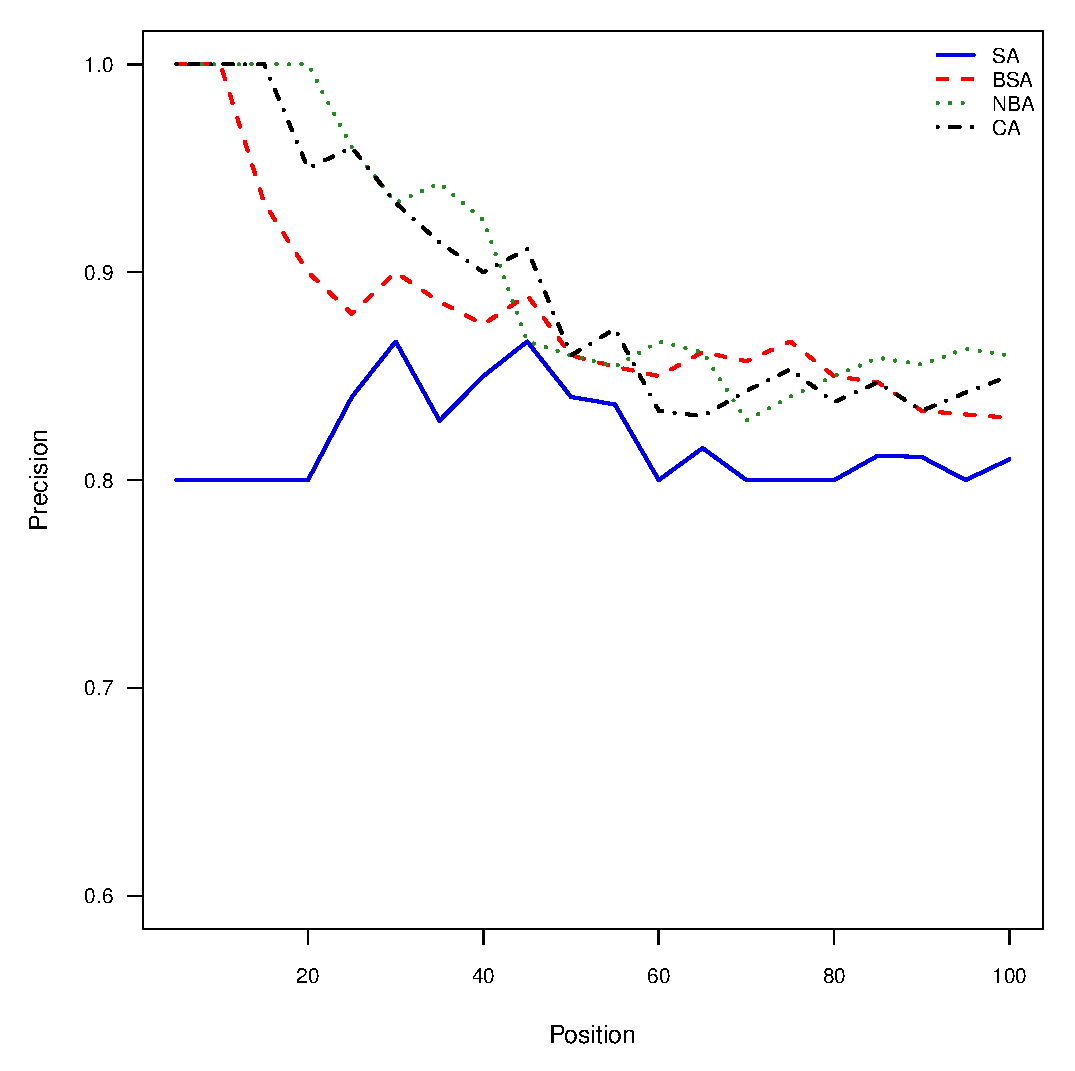
\includegraphics[width=0.45\textwidth]{experiment/e1.ucla.eps}}
\subfigure[MIT]{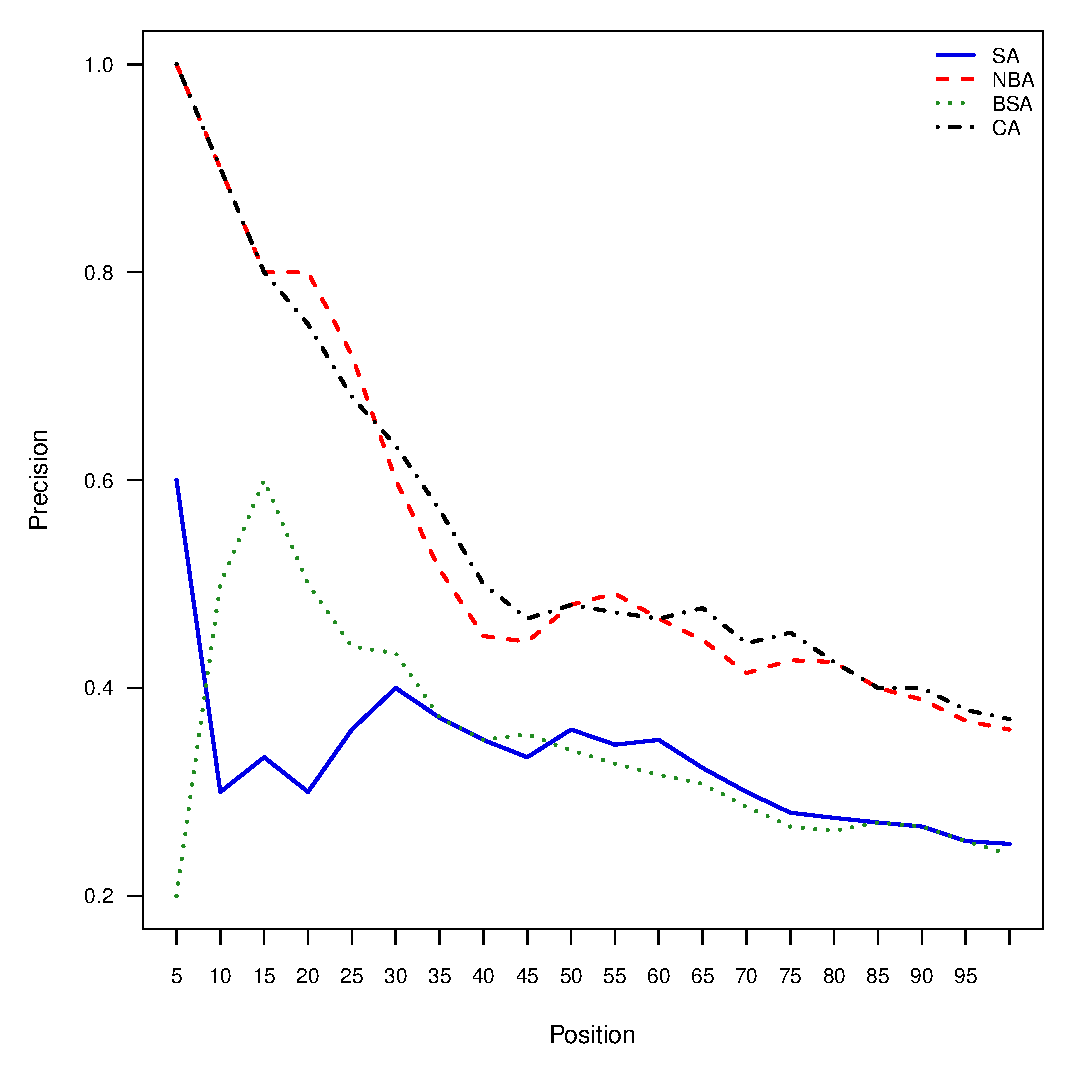
\includegraphics[width=0.45\textwidth]{experiment/e1.mit.eps}}
\\
\subfigure[Stanford]{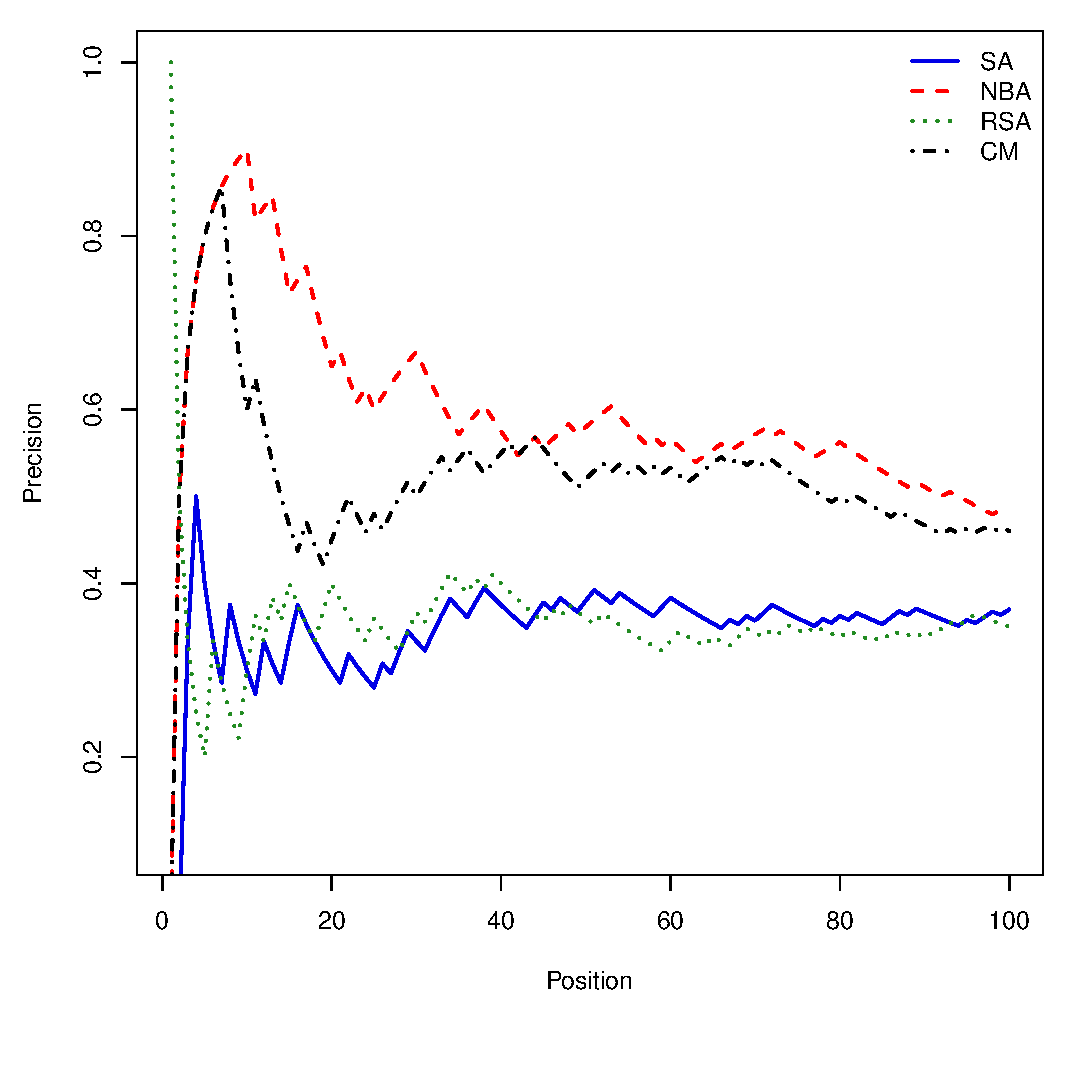
\includegraphics[width=0.45\textwidth]{experiment/e1.stanford.eps}}
\subfigure[USC]{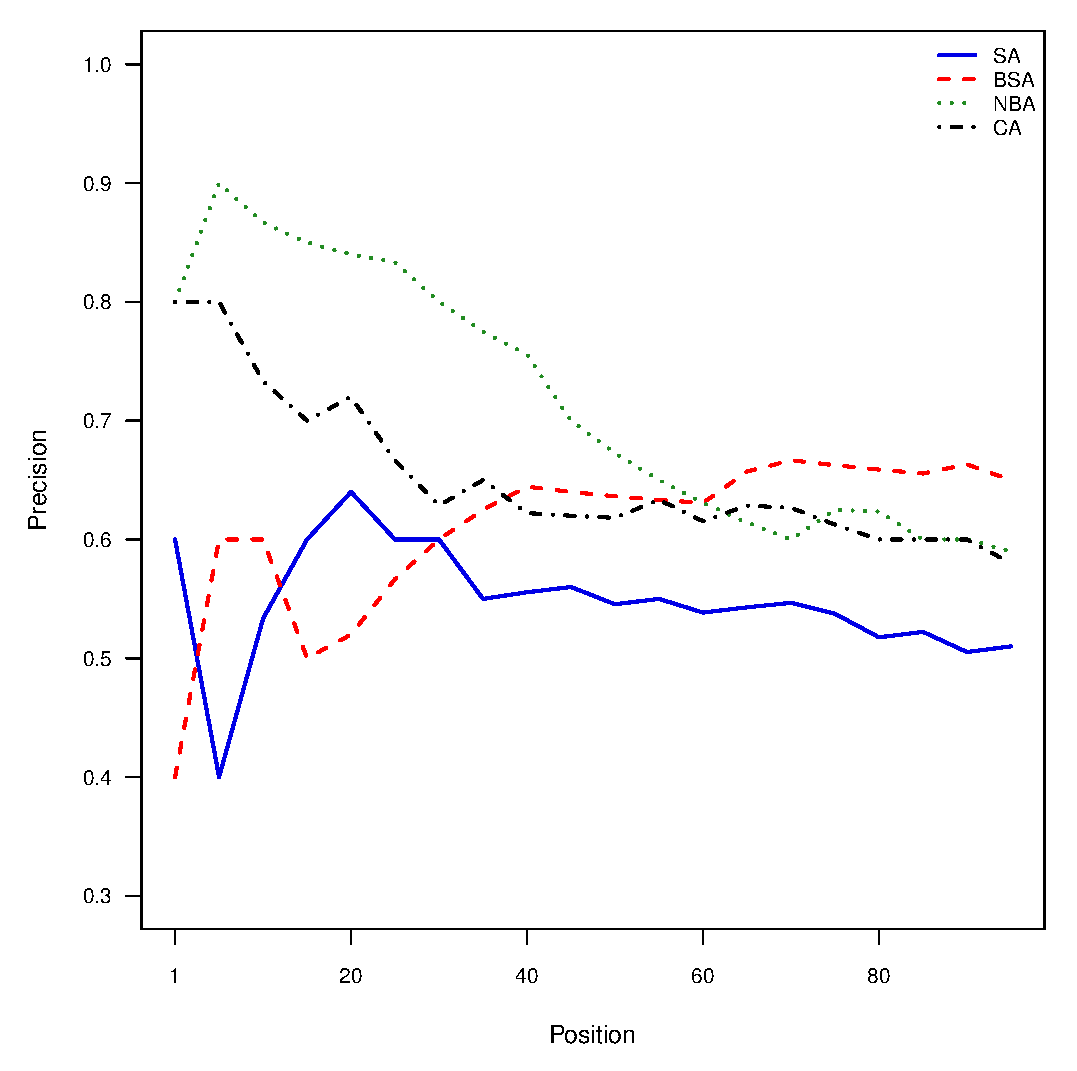
\includegraphics[width=0.45\textwidth]{experiment/e1.usc.eps}}
\caption{Precision\at$k$ for different categories}
\label{fig:e1}
\end{figure*}

From Figure~\ref{fig:e1} we can see that the NBA and CA performs the best at almost every positions. This fact due to the reason that the label data is automated generated by computer. User without category keyword or without large amount of related word will be negative examples in the evaluation. Compare NBA and CA, opposite to our expectation that NBA performs better than CA that is because BSA seriously affected the accuracy of training labels in CA in our computer evaluation system.

The BSA performs better than SA in MIT and USC category, and comparable with SA in Stanford category. But it performs worse than SA in UCLA category, especially in top positions. When we look insight the ranking result, we find that BSA is not as bad as it shows in the figure. For example, the user ranked at the third place in UCLA category is ``LittleBigginKip'', you will find he is a UCLA football team member as soon as you saw his twitter page. However, his profile didn't mention that he is a UCLA student at the time we crawl the data. Moreover, note that much of the improvement in the precision curve in MIT and USC category come in the area after top $10$ positions. This is the area that we most care about, since that users in top position have some features that is easy to discover and users in these middle or tail positions reflect the effectiveness of our algorithm more clearly.

In addition to the keyword based evaluation, Figure~\ref{fig:e2} represents the precision curve in UCLA category on human labeled data. The NBA and CA still performs the best, which shows that users ranked at the top $10$ positions by these algorithms are $100\%$ belong to category UCLA. The BSA performs better than SA since that BSA penalty the users that only interesting to our target category but not actually belong to our target category. For example, the user ``openwestwood'' follows a lot of UCLA stuff which ranked at the $8$th position in SA result but after top 100 positions in BSA result. Actually, after human labeling the experiment result, we find many interesting phenomenons and we will discuss them in our discussion section.
\begin{figure}[htbp]
\centering
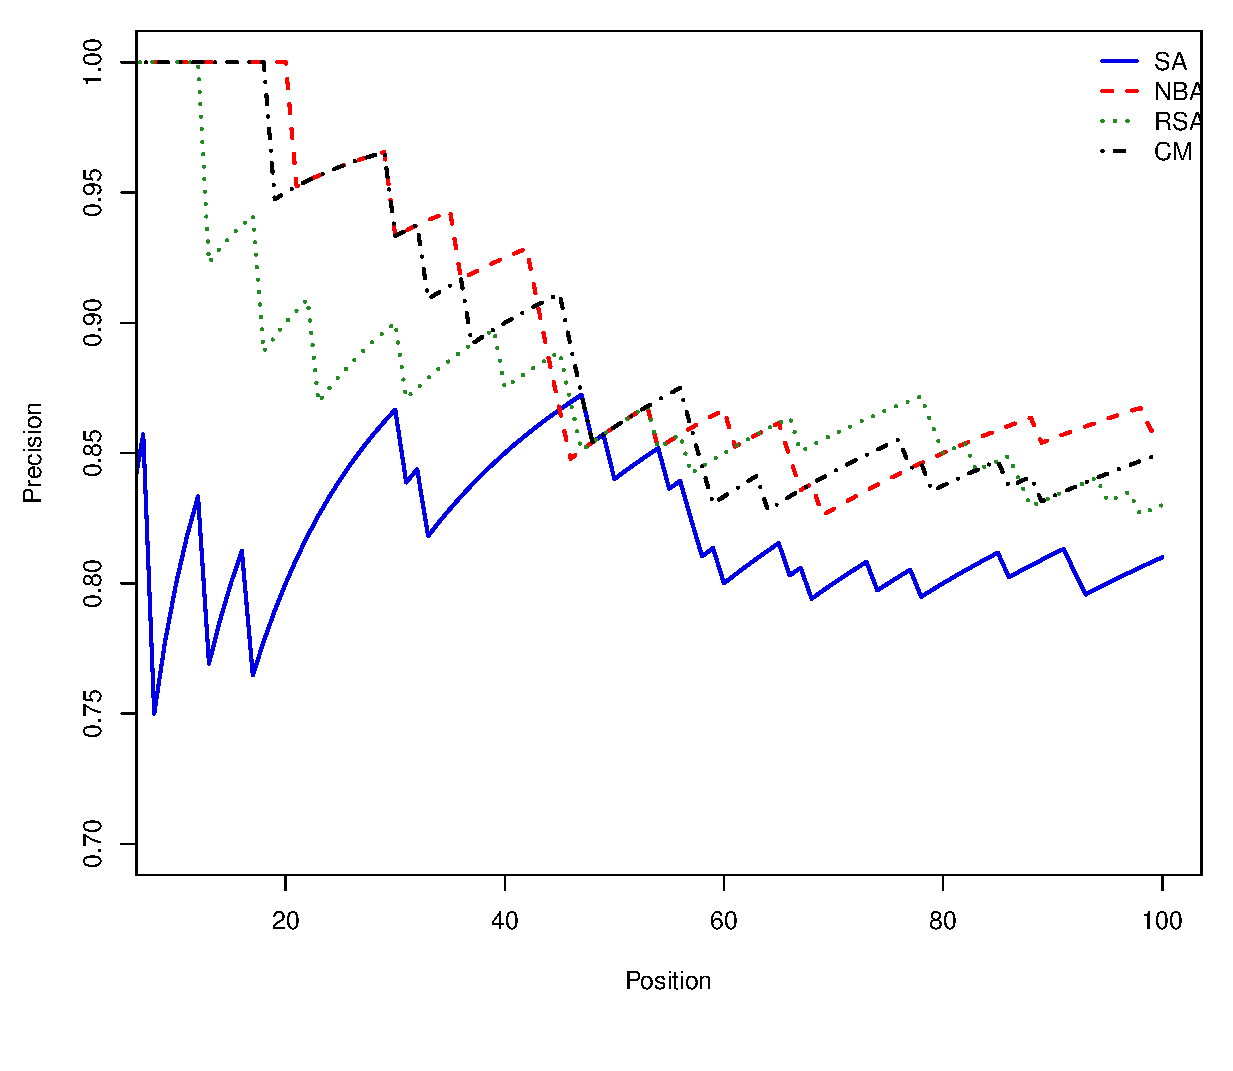
\includegraphics[width=0.45\textwidth]{experiment/e1.ucla.pool.eps}
\caption{Precision\at$k$ for UCLA category on human labeled data}
\label{fig:e2}
\end{figure}

Moreover, we show some important features generated by NBA in Table~\ref{tab:keyword}. The words are ranked according to their occurrence $p(w_i = 1 | c = 1)$, and top 10 words in each category are shown in the table. The top word features for different category are completely different. For example, UCLA students like ``dailybruin'' news, call themselves as ``bruins'' and lived near ``westwood''; USC students like tweets from ``usc annenberge'' and the idol statue in their university is ``Trojan''; MIT students live in ``Cambridge'' and there is famous ``media lab'' in their computer science department; Stanford students are glad to talking about their athletic team using nick name ``cardinal''.

\begin{table*}[htbp]
\centering
\begin{tabular}{|l|l|}
\hline
UCLA & dailybruin, bruin, bruins, westwod, neuheisel, alumna, wooden, undergraduate, midterm, royce \\
\hline
USC & ascj, uscedu, annenberg, uscpsycho, uscannenberg, ausc, beattheirish, trojan, trojans, atrojan \\
\hline
MIT & sloan, medialab, cambridge, joi, kayak, bostonupdate, alums, mechanical, techreview, edu \\
\hline
Stanford & stanfordfball, gostanford, astanford, gsb, cardinal, cantor, tristanwalker, auditorium, alums, freshmen \\
\hline
\end{tabular}
\caption{Top 10 words from user's biography, location and tweets in different universities}\label{tab:keyword}
\end{table*}

\subsection{Ranking with Loss of Information}
In this part of the experiment, the stabilities of different algorithms were tested with loss of information. We randomly selected $1-t\%$ users in $\mathcal{A}$, removed the biography of these users, and moved them to $\mathcal{B}$. The performance of different algorithms under different $t$ is tested, and precision\at$k$ curve is shown in Figure \ref{fig:e3}. SA was not test in this experiment, since its performance is poor in the previous experiment on human labeled data.

\begin{figure}[htbp]
\centering
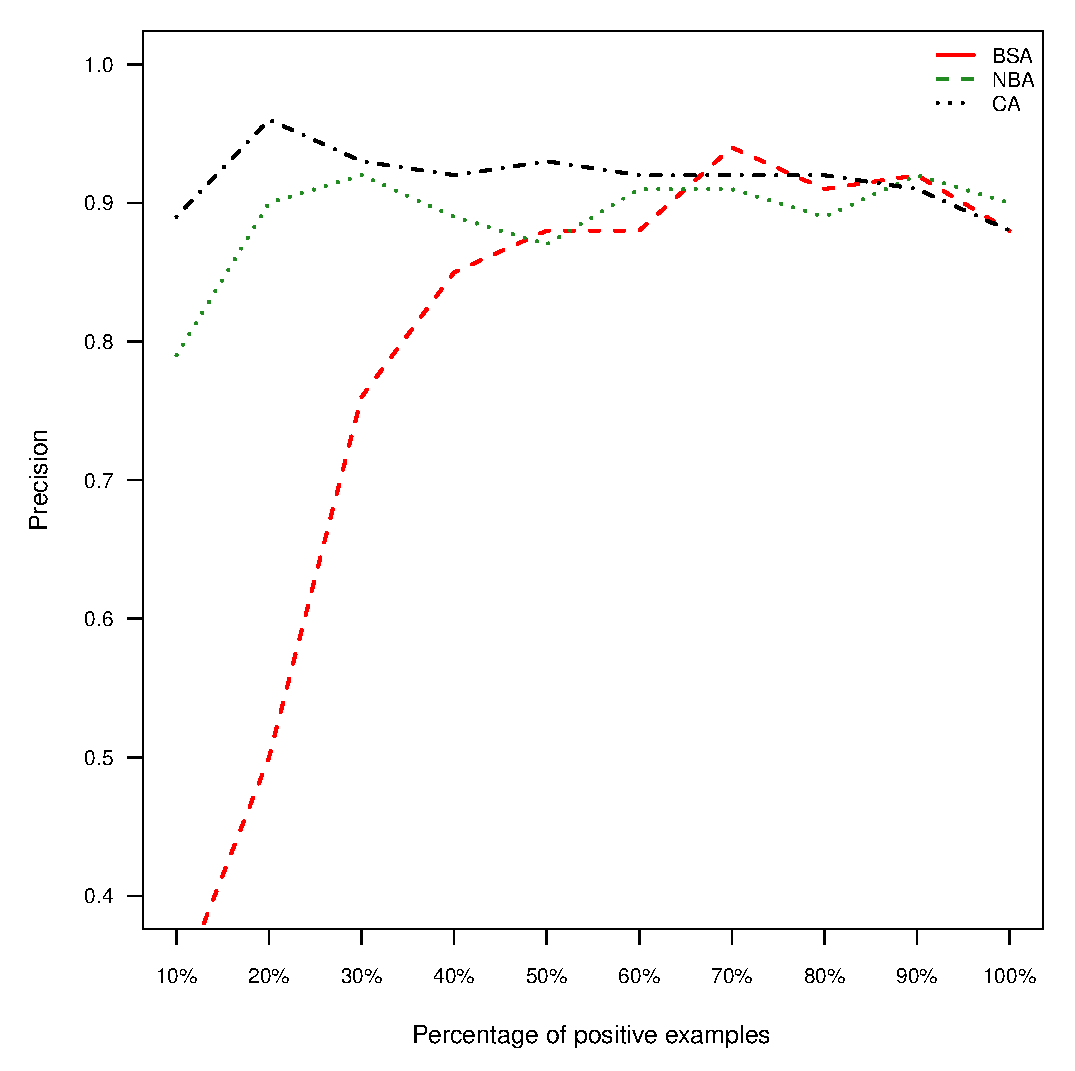
\includegraphics[width=0.45\textwidth]{experiment/e2.ucla.eps}
\caption{Precision\at$k$ for UCLA category with loss of information}
\label{fig:e3}
\end{figure}

The results show that with the loss of information, the performance of BSA falls down dramatically. It also suggests that with few positive training examples, training users in UCLA becomes less connected. The poor graph structure has a bad impact on the performance of BSA.
The NBA still have a very good result with $20\%$ positive training examples. Within those percentage of training users, we could already detect the topic among the tweets published by users belongs to UCLA category. When we look inside the ranking result, the top users returned by BSA and NBA are very accurate. So that the amount of positive training examples does not affect the ranking result of CA very much.

Noticed that sometimes with less positive training examples, our algorithms could achieve better prediction results. That is because when we erase keyword in user's profile, the user is still in our dataset. The total number of users belong to UCLA category in evaluation data increased. So that the precision for top 100 users will be higher.

In our original dataset, the training users are likely to connected with each other since they are in same university. However, for other categories such as father, gamer or phd, users belong to such categories maybe not likely to connected with others in the same category. When we erase the profile keyword in label data, the connection in label data become smaller and the graph structure may like these categories. The performance of our algorithms on UCLA category also demonstrate that our algorithms could be applied to different categories.

\ifx \allfiles \undefined
\end{document}
\fi